\documentclass[14pt, a4paper]{extreport}
\usepackage{susu}

% ====================================================================================================
\begin{document}

\author{Савонин~М.В.}
\group{211}
\task{4}
\maketitle

% ====================================================================================================
\chapter{Задание}

\begin{enumerate}

	\item
	Привести описание и схему алгоритма Брезенхема для растрового представления окружности.

	\item
	Разработать подпрограмму для рисования окружности (аналог процедуры circle из графической библиотеки). Аргументы подпрограммы – координаты 	центра и радиус окружности. При реализации подпрограммы использовать для рисования только процедуру putpixel. Для определения текущего 			цвета рисования использовать функцию getcolor.

	\item
	Разработать подпрограмму для создания фигуры, показанной на рисунке. При создании контура фигуры использовать собственную подпрограмму 			рисования окружности. Для закраски деталей фигуры использовать процедуру floodfill.

	\item
	Написать программу для тестирования разработанных подпрограмм. Интерфейс программы должен содержать следующие элементы управления:
	\begin{itemize}
		\item изменение цвета деталей и фона;
		\item сохранение результата в файл;
		\item выход из программы.
	\end{itemize}

\end{enumerate}

% ====================================================================================================
\chapter{Математическая модель}

Пусть $x_0$, $y_0$, r -- соответственно координаты центра окружности и её радиус.
При рисовании окружности цвет задан изначально color через $COLOR_{MAX}$, а x и y изменения координат пикселей.\\
Рисование окружности:
$$ x = 0 \quad y = r . $$
$$ delta = 3-2*r . $$
$$ mark[2] = [1, -1] . $$
Пока x $\leq$ y выполняем следующие действия:\\
Перебираем i от 0 до 2 не включительно:\\
Перебираем j от 0 до 2 не включительно:\\
Ставим пиксель в точке $x_0$+mark[i]*x, $y_0$+mark[j]*y цвета color.\\
Ставим пиксель в точке $x_0$+mark[i]*x, $y_0$+mark[j]*y цвета color.\\
После всех переборов если p>0 то:
$$ p=p+4*(x-y)+10.  y=y-1$$
Иначе:
$$ p=p+4*x-+6. $$
После чего x=x+1.

% ====================================================================================================
\chapter{Текст программы}

\noindent Файл main.cpp
\lstinputlisting{source/main.cpp}
\pagebreak
\hrulefill

\noindent Файл task.h
\lstinputlisting{source/task.h}
\hrulefill

\noindent Файл task.cpp
\lstinputlisting{source/task.cpp}
\hrulefill

\noindent Файл control.h
\lstinputlisting{source/control.h}
\hrulefill

\noindent Файл control.cpp
\lstinputlisting{source/control.cpp}

% ====================================================================================================
\chapter{Результат работы}

\begin{figure}[h!]
	\centering
	
\includegraphics[width = 12cm]{image/output1}
  \caption{Результат выполнения программы (Пример 1)}
\end{figure}

\begin{figure}[h!]
	\centering
	
\includegraphics[width = 12cm]{image/output2}
  \caption{Результат выполнения программы (Пример 2)}
\end{figure}

\begin{figure}[h!]
	\centering
	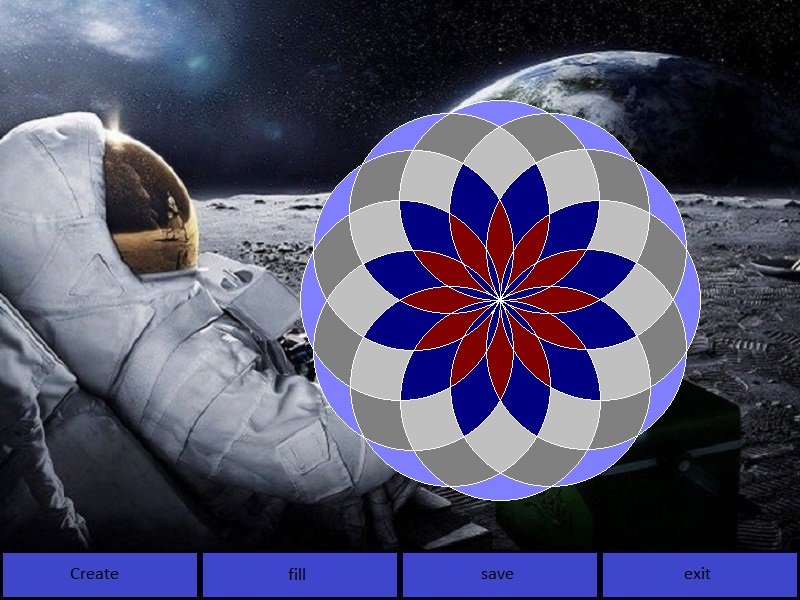
\includegraphics[width = 12cm]{image/output3}
  \caption{Результат выполнения программы (Пример 3)}
\end{figure}

% ====================================================================================================
\end{document}